\section[Gewöhnliche DG II]{Gewöhnliche Differentialgleichungen: Eindeutigkeitssätze, ein Iterationsverfahren und lineare DG im $\mathbb{R}^n$}
\Einleitung{Letzte Woche haben wir uns Lösungsansätze für verschiedene Typen von DG erster Ordnung im $\mathbb{R}^1$ angeschaut.\\
Von dort ausgehend gucken wir nun, welche Bedingungen erfüllt sein müssen, damit genau eine oder mindestens eine Lösung einer DG existiert. Im ersten Fall muss die Funktion $F(x,t)$ der rechten Seite stetig\footnote{Satz von Peano}, im zweiten Fall sogar Lipschitz-stetig\footnote{Satz von Picard-Lindelöf} sein.\\
Aus dem Beweis des Satzes von Picard-Lindelöf fällt zudem ein Iterationsverfahren zur Lösung von DG.\\
Außerdem lernen wir einige auf den ersten (und bestimmt auch den zweiten) Blick komplizierte Verfahren kennen, mit denen wir Lösungen inhomogener, linearer DG-\underline{Systeme} bestimmen können.}

\subsection{Eindeutigkeitssätze für Differentialgleichungen}
Dieses Kapitel wird an späterer Stelle nachgereicht.
\begin{Wiederholung}
{Lipschitzstetigkeit}
Auf \underline{normierten} Räumen $V, W$ und $U\subseteq V$ nennen wir eine Funktion $f:U\to W$ \red{lipschitzstetig} auf $U$, wenn eine Konstante $L\geq 0$ existiert, sodass
\begin{equation*}
    \Norm{f(x)-f(y)}\leq L\Norm{x-y}\quad \forall x,y\in U.
\end{equation*}
\end{Wiederholung}
Für uns ist vor allem folgendes wichtig:
\begin{Satz}{Satz}{Eigenschaften zur Lipschitzstetigkeit}
Lipschitzstetige Funktionen sind \underline{gleichmäßig stetig}.\\
Zudem sind \underline{stetige lineare} Funktionen lipschitzstetig.
\end{Satz}
\blue{Lokale Lipschitzstetigkeit ist also eine ziemlich starke Anforderung an unsere Funktion auf der rechten Seite der DG - mit dieser Forderung können wir aber die Eindeutigkeit der Lösung zeigen.}\\
Zunächst aber noch ein kurzer Satz:
\begin{Satz}
{Satz}{Lipschitzbedingung}
Sei $\Omega=\mathbb{R}^m\times\mathbb{R}$ eine offene Teilmenge.\\
Ist $f:\Omega\to\mathbb{R}$ eine \underline{stetig differenzierbar},
so ist $f$ auf der Teilmenge $K\times[a,b]\subseteq\Omega$ des Urbildes \underline{lipschitzsstetig} bzgl. $x$, wobei $K$ eine \underline{kompakte} und \underline{konvexe} Teilmenge des $\mathbb{R}^n$ ist.
\end{Satz}
\blue{Auf bestimmten Mengen können wir aufgrund dieser Bedingung also die Lipschitzstetigkeit folgern.}
\subsubsection{Picard-Lindelöf}
Der folgende Satz ist DER zentrale Satz des Studiums gewöhnlicher DG.\\
Es werden dabei sehr viele Mengen und Variablen definiert, weshalb ihr ihn Schritt für Schritt durchgehen und ihn am besten direkt mit ein paar Kommilitonen diskutieren solltet.\\
Die Grundaussage ist die folgende:
\begin{Satz}
{Satz}{Satz von Picard-Lindelöf}
Wir betrachten $\Fvec:U\to\mathbb{R}^n$.\\
Auf einer Teilmenge $Q\subseteq U$, auf der $\Fvec$ bzgl. $\xvec$ \underline{lipschitzstetig} ist, hat das AWP $\boxed{\xvec'=\Fvec(\xvec,t)}$ mit $\xvec(t_0)=\xvec_0$ \underline{genau eine} $C^1$-Lösung\footnote{also stetig differenzierbar} $\xvec:I\to\mathbb{R}^n$.
\end{Satz}
\textbf{Genauere Betrachtung:}\\
Die Art des Intervalls $I$ gucken wir uns jetzt genauer an:\\
Die Funktion $\Fvec:U\to\mathbb{R}^n$ bildet wieder die rechte Seite der DG, wobei $U\subseteq \mathbb{R}^n\times t$ ist.\\
Die Teilmenge $Q$, auf der $\Fvec$ lipschitzstetig sein soll, wählen wir als abgeschlossene Kugel um die Anfangswerte.\\
Das sieht dann so aus:\\ $Q:=\overline{B_\bvec(\xvec_0)}\times[t_0-a,t_0+a]\subseteq U$ mit $a,b>0$, wobei wir also quasi zwei abgeschlossene Kugeln haben: Eine Kugel mit Radius $b$ um $\xvec$ und eine 'Kugel' mit Radius $a$ um $t_0$.\\
Um das Intervall $I$ (für $t$) zu bestimmen, auf dem die Lösung des AWP eindeutig ist, betrachten wir das Maximum der Funktionswerte, die $\Fvec$ auf $Q$ annimmt:\\
$M:=\max_{(\yvec, t)\in Q}\Norm{F(\yvec,t)}$ und die Lipschitzkonstante $L$.\\
Die Grenzen für das Intervall $I$ sind dann $I=[t_0-\sigma, t_0+\sigma]$, wobei $\sigma=\min\BracedIn{a,\frac{b}{M},\frac{1}{2L}}$ ist.\\
Alle Funktionswerte der Lösung $\xvec:I\to\mathbb{R}^n$ liegen dann innerhalb $\overline{B_\bvec(\xvec_0)}$.\\
\blue{Zum Beweis:\\
Der Beweis verwendet den Banachschen Fixpunktsatz, welcher folgende Aussage machte:}
\begin{Wiederholung}
{Banachscher Fixpunktsatz}
Für jede kontrahierende Abbildung\footnote{also eine Abbildung, für die $d(F(x),F(y))\leq\theta d(x,y)$ mit $0\leq\theta<1$ gilt - man könnte auch sagen, dass sie lipschitzstetig mit der Lipschitzkonstante $L<1$ sein muss.} in einem \underline{vollständigen}\footnote{Wdh.: In einem vollständigen Raum konvergiert jede Cauchy-Folge gegen ein Element aus diesem Raum.} metrischen Raum $(X,d)$ existiert ein \underline{eindeutiger} \red{Fixpunkt} $\Tilde{x}\in X$.\\
Für diesen gilt, dass $\boxed{F(\Tilde{x})=\Tilde{x}}$.\\
Zudem konvergiert die Folge $\boxed{x_{k+1}=F(x_k)}$ für alle Anfangswerte $x_0\in X$ gegen den Fixpunkt, $\lim_{n\to\infty}x_n=\Tilde{x}$.
\end{Wiederholung}
\blue{Die Beweisidee des Satzes von Picard-Lindelöf ist nun, als vollständigen metrischen Raum $X$ aus dem Fixpunktsatz folgenden Raum zu wählen:
\begin{equation*}
    (X,\Norm{\cdot}_\infty)=\Menge{\xvec:I\to\mathbb{R}^n}{\xvec\tx{ ist stetig}},\quad I=[t_0-\sigma,t_0+\sigma]
\end{equation*}
wobei $\Norm{f}_\infty=\sup_{t\in I}(\xvec(t))$ die Supremumsnorm ist.\\
Für die Lösung des AWP $\xvec'=\Fvec(\xvec,t)$ wird nun auf beiden Seiten integriert.\\
Formell ist dann schon
\begin{equation*}
    \xvec(t)=\xvec_0+\int_{t_0}^t\Fvec(\xvec(s),s)ds
\end{equation*}
eine Lösung.\\
Wir wollen nun zeigen, dass diese eindeutig ist. Dafür nutzen wir den Fixpunktsatz, aber vorher benötigen wir ja noch unsere kontrahierende Abbildung.\\
Diese definieren wir uns als Abbildung zwischen Räumen der stetigen Funktionen:
\begin{equation*}
    H:C(I,\overline{B_\bvec(\xvec_0)})\to C(I,\mathbb{R}^n),\quad\xvec\mapsto H(\xvec):t\mapsto\xvec_0+\int_{t_0}^t\Fvec(\xvec(s),s)ds.
\end{equation*}
Die Abbildung $H$, die wir auch als \red{Integraloperator} bezeichnen, bildet eine Funktion $\xvec$ also auf eine weitere von $t$ abhängige Funktion, nämlich genau deren Integral mit Integrationskonstante $\xvec_0$, ab.\\
Für die Eindeutigkeit der Lösung müssen wir zeigen, dass der Integraloperator die Lösung unverändert lässt, also einen Fixpunkt besitzt, für den $H(\xvec(t))=\xvec(t)$ gilt.\\
Im \Skript{} (F. 360-362) seht ihr, dass $H$ kontrahierend und die damit gefundene Lösung also eindeutig ist.}

\subsubsection{Ein Iterationsverfahren}
Kurioserweise liefert der im Beweis verwendete Banachsche Fixpunktsatz nun auch eine Vorschrift, mit der wir uns dem Fixpunkt des Integraloperators und damit der Lösung $\varphivec(t)$ eines AWP $\xvec'=\Fvec(\xvec,t)$ (sofern die Voraussetzungen erfüllt sind) nähern können.
\begin{Satz}
{Lösungsansatz}{Iterationsverfahren von Picard-Lindelöf}
Wir betrachten ein AWP $\xvec'=\Fvec(\xvec,t)$, für das $\Fvec:U\to\mathbb{R}^n$ stetig ist und zudem die weiteren Voraussetzungen des Satzes von Picard-Lindelöf (Lipschitzstetigkeit auf Einschränkung $Q$ usw.) erfüllt sind.\\
Dieses AWP können wir folgendermaßen iterativ lösen:
\begin{itemize}
    \item Als Startpunkt wählen wir $\varphivec_0(t)=\xvec_0$.
    \item Die verwendete Abbildung ist der Integraloperator $H$, also ist das nächste Folgenglied gegeben durch
    \begin{equation*}
        \varphivec_1(t)=H(\varphivec_0(t))=\xvec_0+\int_{t_0}^t\Fvec(\varphivec_0(s),s)ds.
    \end{equation*}
    \item Das $n$-te Folgenglied ist dann auch einfach gegeben:
    \begin{equation*}
        \varphivec_n(t)=H(\varphivec_{n-1}(t))=\xvec_0+\int_{t_0}^t\Fvec(\varphivec_{n-1}(s),s)ds.
    \end{equation*}
\end{itemize}
Der Fehler dieser gleichmäßig gegen die Lösung $\xvec(t)$ konvergierenden Funktionenfolge kann zu
\begin{equation*}
    \Norm{\xvec(t)-\varphivec_n(t)}_\infty\leq\frac{b}{2^n}
\end{equation*}
oder für $t\in I=[t_0-\sigma,t_0+\sigma]$ sogar zu
\begin{equation*}
    \Norm{\xvec(t)-\varphivec_n(t)}_\infty\leq\frac{ML^n}{(n+1)!}\Abs{t-t_0}^{n+1}
\end{equation*}
abgeschätzt werden.
\end{Satz}
\blue{
Letztes Mal hatten wir gesehen, dass wir DG höherer Ordnung mit simplen Mitteln auf ein System aus DG} erster Ordnung reduzieren konnten.
\begin{Beispiel}
{AWP mit Iterationsrverfahren}
Wir betrachten dementsprechend $\boxed{x''=x-kx'+t}$ mit $x(0)=1$ und $x'(0)=0$.\\
Der Reduktionstrick war nun, die zweite Ableitung als Ableitung der ersten auszudrücken.\\
Wir setzen daher $y_1=x$ und $y_2=x'$, sodass (mithilfe der DG)
\begin{equation*}
    \yvec'=\Matrix{y_1'\\y_2'}=\Matrix{x'\\x''}=\Matrix{y_2\\y_1-ky_2}+\Matrix{0\\t}=\Matrix{0&1\\1&-k}\Matrix{y_1\\y_2}+\Matrix{0\\t}.
\end{equation*}
In Kurzschreibweise haben wir also $\boxed{\yvec'=\MatrixInline{0&1\\1&-k}\yvec+\MatrixInline{0\\t}}=\Fvec(\yvec(t),t)$ mit der AB\\
$\yvec(0)=\MatrixInline{1\\0}$.\\
Dies können wir also iterativ lösen.
\begin{itemize}
    \item Wir nutzen $\varphivec_0(t)=\yvec_0=\MatrixInline{1\\0}$.
    \item Damit ist
    \begin{align*}
        \varphivec_1(t)&=H(\varphivec_0(t))=\yvec_0+\int_{t_0}^t\Fvec(\varphivec_0(s),s)ds\\
        &=\Matrix{1\\0}+\int_0^t\BracedInSqr{\Matrix{0&1\\1&-k}\overbrace{\Matrix{1\\0}}^{\varphivec_0(s)}+\Matrix{0\\s}}ds\\
        &=\Matrix{1\\0}+\int_0^t\Matrix{0\\1+s}ds=\Matrix{1\\t+\frac{t^2}{2}}.
    \end{align*}
    \item Das zweite Glied dieser Folge ist somit
    \begin{align*}
        \varphivec_2(t)&=\Matrix{1\\0}+\int_0^t\BracedInSqr{\Matrix{0&1\\1&-k}\Matrix{1\\s+\frac{s^2}{2}}+\Matrix{0\\s}}ds\\
        &=\Matrix{1\\0}+\int_0^t\Matrix{s+\frac{s^2}{2}\\1-ks+s-k\frac{s^2}{2}}ds=\Matrix{1+\frac{t^2}{2}+\frac{t^3}{1\cdot2\cdot3}\\t+\frac{t^2}{2}-k\BracedIn{\frac{t^2}{2}+\frac{t^3}{3!}}}.
    \end{align*}
    \item Langsam wird's kompliziert. Das nächste Glied ist
    \begin{equation*}
        \varphivec_3(t)=\Matrix{1\\0}+\int_0^t\Matrix{s+\frac{s^2}{2}-k\BracedIn{\frac{s^2}{2!}+\frac{s^3}{3!}}\\1+s+\frac{s^2}{2!}+\frac{s^3}{3!}-k\BracedInSqr{s+\frac{s^2}{2}-k\BracedIn{\frac{s^2}{2!}+\frac{s^3}{3!}}}}ds=\ldots
    \end{equation*}
\end{itemize}
In diesem Fall würde man also nur eine approximative Lösung bekommen, die mit jedem Iterationsschritt komplizierter aussieht.
\end{Beispiel}
\blue{In gewissen Fällen kann man bei genügend Iterationen die einzelnen Komponenten aber auch als Reihen aufschreiben:}
\begin{Beispiel}
Wir betrachten das AWP $x''=x+t$ mit $x(0)=1,\,x'(0)=0$, was wir mit $y_1=x,\,y_2=x'$ und $y_2'=x''=x+t=y_1+t$ zurückführen können auf
\begin{equation*}
    \boxed{\yvec'=\overbrace{\Matrix{0&1\\1&0}\yvec+\Matrix{0\\t}}^{\Fvec(\yvec(t),t)}},\quad \yvec(0)=\Matrix{1\\0}.
\end{equation*}
Wir suchen die Lösung wieder iterativ\footnote{Bei dieser DG handelt es sich um eine inhomogene lineare DG, die wir auch mit einer Fundamentalmatrix lösen könnten, siehe Kap. \ref{sssec:12InhomogeneSysteme}}:
\begin{itemize}
    \item Wir nutzen $\varphivec_0(t)=\Matrix{1\\0}$.
    \item Dann ist
    \begin{equation*}
        \varphivec_1(t)=\yvec_0+\int_0^t\Fvec(\varphivec_0(s),s)ds=\Matrix{1\\0}+\int_0^t\BracedInSqr{\Matrix{0&1\\1&0}\Matrix{1\\0}+\Matrix{0\\s}}ds=\Matrix{1\\t+\frac{t^2}{2}}.
    \end{equation*}
    \item Weiterhin ist
    \begin{equation*}
        \varphivec_2(t)=\Matrix{1\\0}+\int_0^t\Matrix{s+\frac{s^2}{2}\\1+s}ds=\Matrix{1+\frac{t^2}{1\cdot 2}+\frac{t^3}{1\cdot2\cdot3}\\t+\frac{t^2}{2!}}.
    \end{equation*}
    \item Die nächste Iteration ergibt
    \begin{equation*}
        \varphivec_3(t)=\Matrix{1\\0}+\int_0^t\Matrix{s+\frac{s^2}{2!}\\1+s+\frac{s^2}{2!}+\frac{s^3}{3!}}ds=\Matrix{1+\frac{t^2}{2!}+\frac{t^3}{3!}\\t+\frac{t^2}{2}+\frac{t^3}{3!}+\frac{t^4}{4!}}.
    \end{equation*}
    \item So geht das auch weiter... Erkennt ihr ein Muster?
\end{itemize}
Bei genauerem Hinschauen erinnert dies an die Exponentialfunktion 
\begin{equation*}
    e^x=\sum_{k=0}^\infty\frac{x^k}{k!}=1+x+\frac{x^2}{2}+\frac{x^3}{3!}+\ldots.
\end{equation*}
Tatsächlich konvergiert die Lösung dieses AWPs gegen
\begin{equation*}
    \varphivec(t)=\Matrix{e^t-t\\e^t-1},
\end{equation*}
denn dies erfüllt die DG:
\begin{equation*}
    \varphivec'(t)=\Matrix{e^t-1\\e^t}=\Matrix{0&1\\1&0}\Matrix{e^t-t\\e^t-1}+\Matrix{0\\t}=\Matrix{0&1\\1&0}\varphivec(t)+\Matrix{0\\t}.
\end{equation*}
\end{Beispiel}

\subsubsection{Weitere Eindeutigkeitsaussagen}
\begin{Satz}
{Satz}{Eindeutigkeitssatz}
Wir betrachten $\Omega\subseteq \mathbb{R}^n\times \mathbb{R}$.\\
Sei $\Fvec:\Omega\to\mathbb{R}^n$ \underline{stetig} und bzgl. $\xvec$ lokal \underline{lipschitzstetig}.\\
Liegen zwei Lösungen $\varphivec,\psivec:I=(a,b)\to\mathbb{R}^n$ von $\xvec'=\Fvec(\xvec,t)$ vor, die das AWP $\varphivec(t_0)=\psivec(t_0)=\xvec_0$ für $t_0\in I$ lösen, so handelt es sich um dieselben Lösungen, $\varphivec=\psivec$.
\end{Satz}

Der folgende Satz hat eine nicht ganz so schöne Aussage wie der Satz von Picard-Lindelöf, dafür aber deutlich schwächere Forderungen, denn $\Fvec$ muss nur stetig, aber \underline{nicht} lipschitzstetig sein.
\begin{Satz}
{Satz}{Existenzsatz von Cauchy und Peano}
Seien die Voraussetzungen wie für den Satz von Picard-Lindelöf, außer, dass $\Fvec$ auf dem kompakten Bereich $Q$ nur stetig, aber nicht unbedingt lipschitzstetig sei.\\
Dann hat das AWP $\xvec'=\Fvec(\xvec,t),\quad \xvec(t_0)=\xvec_0$ \underline{mindestens eine} stetig differenzierbare Lösung $\xvec:[t_0-\sigma, t_0+\sigma]\to\mathbb{R}^n$.
\end{Satz}

\subsubsection{Abhängigkeit der Lösungen von den Anfangsbedingungen}
\blue{Wir wollen nun genauer betrachten, was passieren kann, wenn wir die Anfangsbedingung unserer DG variieren - in vielen Fällen kommen Fallunterscheidungen auf uns zu.\\
Liegt auf der rechten Seite der DG jedoch eine lipschitzstetige Funktion vor, so können wir folgern, dass auf kompakten Intervallen $I$ (wo $t$ herkommt) die Folge der Lösungen $\varphivec_{\xvec_n}(t)$ mit einer gegen $\lim_{n\to\infty}\xvec_n=\xvec_0$ konvergierenden Folge von Anfangsbedingungen auch gegen die Lösung $\varphivec_{\xvec_0}(t)$ konvergiert.}\\
Mitunter müssen wir bei der Lösung also aufpassen.
\begin{Beispiel}
{Betrachtung eines Vektorfelds}
Wir betrachten das Vektorfeld $V:\mathbb{R}^2\to\mathbb{R}^2,\,V(x,y)=\MatrixInline{x^2\\\sqrt{1-y^2}}$.\\
Wir suchen nun alle Integralkurven $\gamma$ von $V$, die der AB $\gamma(0)=\MatrixInline{x_y\\y_0}$ (mit $x_0\neq0,\,y\in[-1,1]$ genügen.\\
Dann gilt: $\gamma'=V(\gamma)$.\\
Wir schreiben $\gamma$ als $\gamma=\MatrixInline{x\\y}$.\\
Dann ist $x'=x^2$ und $y'=\sqrt{1-y^2}$.\\
Dies sind zwei autonome DG, deren Lösung
\begin{equation*}
    \gamma(t)\overset{*}{=}\Matrix{\frac{x_0}{1-x_0t}\\\sin(t-\arcsin(y_0))}
\end{equation*}
ist, wobei wir in einer NR gesehen haben, dass 
\begin{align*}
    \int_{x_0}^x\frac{dx}{x^2}&=\int_{t_0}^tdt\\
    \iff -\frac{1}{x}+\frac{1}{x_0}&=t-0\implies x(t)=-\frac{1}{t-1/x_0}=\frac{x_0}{1-x_0t}
\end{align*}
und\footnote{mit $y(x)=\arcsin(x)\iff \sin(y)=x\implies y'\cos(y)=1\implies y'(x)=\frac{1}{\sqrt{1-\sin^2(y)}}=\frac{1}{\sqrt{1-x^2}}$}
\begin{align*}
    \int_{y_0}^y\frac{dy}{\sqrt{1-y^2}}&=\int_{t_0}^tdt\\
    \arcsin(y)-\arcsin(y_0)&=t\implies y(t)=\sin(t-\arcsin(y_0)).
\end{align*}
\textbf{Was ist nun der Definitionsbereich?}\\
der Sinus isf ür alle Argumente definiert, der einzig kritische Punkt tritt bei $t=x_0$ auf.\\
Der maximale Definitionsbereich ist also $\mathbb{R}\setminus\MengeDirekt{\frac{1}{x_0}}$.\\
Um die Lösung zu skizzieren, wählen wir verschiedene feste Paare $(x_0,y_0)$ und dann jeweils verschiedene Zeitabschnitte.\\
Für $x_0=1,\,y_0=0$ sieht das dann so aus:
\begin{center}
    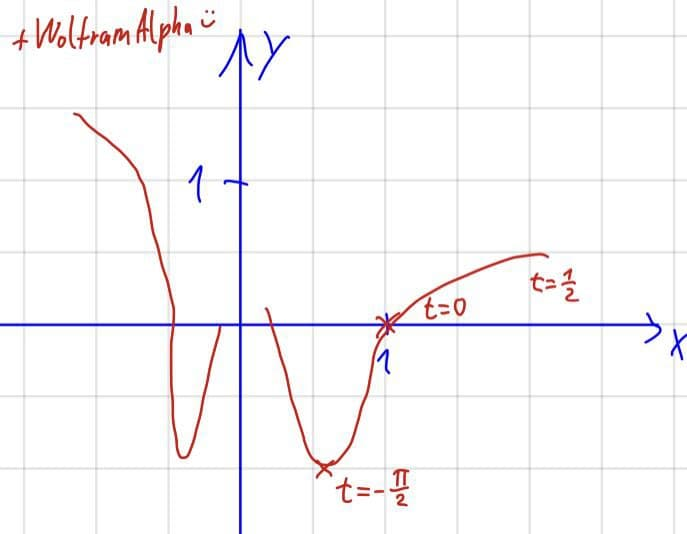
\includegraphics[width=.35\textwidth]{Dateien/12Vektorfeld.jpg}
\end{center}
Was passiert bei Variation der AB?
\begin{itemize}
    \item Variation von $x_0$ führt zu einer Verschiebung der Integralkurve nach links oder rechts.
    \item Variation von $y_0$ führt zu einer Verschiebung nach oben oder unten.
\end{itemize}
\end{Beispiel}


\subsection[Systeme linearer DG]{Systeme linearer DG im $\mathbb{R}^n$}
Wir betrachten nun \underline{lineare} Systeme von Differentialgleichungen im $\mathbb{R}^n$, deren Spezialfall wir im $\mathbb{R}^1$ schon kennengelernt hatten.\\
Hier lautete die DG $x'=p(t)x+q(t)$ mit einem homogenen und einem inhomogenen Anteil.\\
Wir hatten gesehen, dass Linearkombinationen aus homogener und spezieller Lösung auch wieder eine \textit{allgemeine} Lösung bilden.\\
Wie sieht das nun aber aus, wenn $\xvec\in \mathbb{R}^n$ ein Vektor ist?
\begin{Satz}
{Satz}{Lösungen homogener linearer DG bilden einen Vektorraum}
Liegt ein lineares homogenes System
\begin{equation*}
    \xvec'=A(t)\xvec
\end{equation*}
vor, so ist die Menge der maximalen Lösungen $\xvec:I\to\mathbb{R}^n$ ein $n$-dimensionaler, reeller Vektorraum.\\
\blue{Linearkombinationen von Lösungen sind also auch wieder Lösungen.}
\end{Satz}
\begin{Satz}
{Satz}{Lösungen inhomogener linearer DG bilden einen affinen Raum}
Liegt ein lineares System mit Inhomogenität $\bvec(t)$
\begin{equation*}
    \xvec'=A(t)\xvec+\bvec(t)
\end{equation*}
vor, so bildet der affine Raum $\mathcal{A}=\xvec_s+V$ (wobei $\xvec_s$ eine spezielle Lösung und $V$ der Lösungsraum des homogenen Systems sind) die maximale Lösungsmenge.
\end{Satz}
Dieses Verhalten hatten wir auch schon im $\mathbb{R}^1$ beobachtet, wo $A(t)=p(t)$ und $b(t)=q(t)$ waren. Auch hier war ja eine Kombination von allgemeiner und spezieller Lösung wieder eine Lösung.\\
Wir können nun auf Werkzeuge zurückgreifen, die wir im Zusammenhang mit Vektorräumen definiert hatten.
\begin{Def}
{Fundamentalsystem{,} Fundamentalmatrix und Wronski-Determinante}
Weil wir wissen, dass der Lösungsraum des homogenen, linearen DG-Systems $\xvec'=A(t)\xvec$ ein Vektorraum ist, muss dieser eine Basis $\mathcal{B}=(\varphivec_1,\ldots,\varphivec_n)$ besitzen. Diese Basis nennen wir \red{Fundamentalsystem}.\\
Die $\varphivec_j$ sind dabei Spaltenvektoren, aus denen wir die \red{Fundamentalmatrix}
\begin{equation*}
    \Phi =\Matrix{\varphivec_1&\cdots&\varphivec_n}
\end{equation*}
konstruieren können.\\
Deren Determinante $\det\Phi$, die \red{Wronski-Determinante}, gibt uns Auskunft darüber, ob wir mit den $\varphivec_j$ wirklich ein Fundamentalsystem, also eine Basis des Lösungsraums gefunden haben.
\end{Def}
\begin{Satz}
{Satz}{Zur Wronski-Determinante}
Existiert $t$, sodass $W=\det\Phi\neq0$ ist (wobei $\Phi=\MatrixInline{\varphivec_1(t)&\cdots&\varphivec_n(t)}$), so handelt es sich bei $\Phi$ um eine Fundamentalmatrix.\\
Es gilt $\Phi'=A(t)\Phi$, denn $\Phi'=\Matrix{\varphivec'_1&\cdots&\varphivec'_n}=\Matrix{A\varphivec_1&\cdots&A\varphivec_n}=A\Phi$.
\end{Satz}
Wozu ist $\Phi$ nun gut?
\begin{Satz}
{Lösungsansatz}{Lösung eines homogenen linearen Anfangswertproblems}
Mithilfe der Fundamentalmatrix können wir Lösungen homogener AWP der Form $\xvec'=A(t)\xvec$ mit $\xvec(t_0)=\xvec_0$ bestimmen.\\
Diese ist gegeben durch
\begin{equation*}
    \varphivec(t)=\Phi(t)\BracedIn{\Phi(t_0)}^{-1}\xvec_0.
\end{equation*}
\end{Satz}
\begin{Beispiel}
{Homogenes lineares Anfangswertproblem}
Wir betrachten das homogene lineare System
\begin{equation*}
    \Matrix{x_1\\x_2}'=\overbrace{\Matrix{0&-\omega\\\omega&0}}^{=:A}\Matrix{x_1\\x_2},\quad \xvec\BracedIn{\frac{\pi}{2\omega}}=\Matrix{0\\1}.
\end{equation*}
Eine Fundamentalmatrix ist gegeben durch (s. a. F. 385 im \Skript{}, Ansätze, wie man sie finden würde, sind im nächsten Kapitel geschildert)
\begin{equation*}
    \Phi(t)=\Matrix{\cos(\omega t)&-\sin(\omega t)\\\sin(\omega t)&\cos(\omega t)},
\end{equation*}
denn es gilt
\begin{equation*}
    \Phi'=\Matrix{-\omega\sin(\omega t)&-\omega\cos(\omega t)\\\omega\cos(\omega t)&-\omega\sin(\omega t)}=\Matrix{0&-\omega\\\omega &0}\Matrix{\cos(\omega t)&-\sin(\omega t)\\\sin(\omega t)&\cos(\omega t)}=A\Phi.
\end{equation*}
Die Lösung des AWP ist also (mit $t_0=\frac{\pi}{2\omega}$) gegeben durch
\begin{align*}
    \varphivec(t)&=\Phi(t)\BracedIn{\Phi(t_0)}^{-1}\xvec_0=\Matrix{\cos(\omega t)&-\sin(\omega t)\\\sin(\omega t)&\cos(\omega t)}\Matrix{\cos(\omega t_0)&-\sin(\omega t_0)\\\sin(\omega t_0)&\cos(\omega t_0)}^{-1}\Matrix{0\\1}\\
    &=\Matrix{\cos(\omega t)&-\sin(\omega t)\\\sin(\omega t)&\cos(\omega t)}\Matrix{0&-1\\1&0}^{-1}\Matrix{0\\1}\\
    &=\Matrix{\cos(\omega t)&-\sin(\omega t)\\\sin(\omega t)&\cos(\omega t)}\Matrix{1\\0}=\Matrix{\cos(\omega t)\\\sin(\omega t)},
\end{align*}
wobei wir die Cramersche Regel genutzt haben, um zu sehen, dass $\MatrixInline{0&-1\\1&0}^{-1}=\MatrixInline{0&1\\-1&0}$.
\end{Beispiel}
\subsubsection{Bestimmung der Fundamentalmatrix}
Bevor wir uns den inhomogenen linearen DG-Systemen widmen, stellt sich zunächst die Frage, wie man diese überhaupt bestimmt.\\
Dafür schränken wir uns auf den Spezialfall einer Matrix $A(t)=A$ mit \red{konstanten Koeffizienten} ein.\\
\blue{\textbf{Motivation mithilfe von eindimensionalen DG}:\\
Wir erinnern uns zurück an das 1D-AWP $x'=p(t)x+q(t)$ mit $x(t_0)=x_0$.\\
Hier haben wir die homogene Lösung durch Trennung der Variablen bestimmt:
\begin{align*}
    x'(t)=p(t)x&\iff \int_{x_0}^x\frac{dz}{z}=\int_{t_0}^tp(s)ds\\
    &\iff \ln(x)-\ln(x_0)=\int_{t_0}^tp(s)ds\\
    &\iff x(t)=x_0\exp\BracedIn{\int_{t_0}^tp(s)ds}.
\end{align*}
Im Falle einer konstanten Funktion $p(t)=p=const.$ ist die Lösung einfach $x(t)=x_0e^{p(t-t_0)}$.\\
Wenn ihr den letzten Abschnitt aufmerksam gelesen habt, sollte euch das bekannt vorkommen.\\
Tatsächlich wäre die Exponentialfunktion $\Phi(t)=\Matrix{e^{pt}}$ hier dann eine Fundamentalmatrix.\\
Der einzige Basisvektor des Lösungsraumes wäre $\varphi_1=e^{pt}$ und beliebige Linearkombinationen (welche aufgrund der Eindimensionalität nur Vielfachen entsprechen) sind wieder Lösungen der DG $x'=px$.\\
Ist unsere DG jetzt mehrdimensional,  d. h. $\xvec'=A\xvec$, dann ist die Lösung auch nichts weiter als $\Phi(t)=e^{At}$ und beliebige Linearkombinationen sind auch wieder Lösungen.\\
Dafür wird das Matrixexponential analog zur 1D-Exponentialfunktion definiert.}\\
\blue{Wie wir im folgenden Abschnitt sehen werden, kommt man über das Picard-Lindelöf'sche Iterationsverfahren auf diese Lösung.\\
Die konkrete Lösung zum AWP ist dann $\varphivec(t)=\Phi(t)\BracedIn{\Phi(t_0)}^{-1}\xvec_0=e^{A(t-t_0)}\xvec_0$.\\
Seht ihr die Analogie zum 1D-Fall?}
\begin{Def}
{Matrixexponential}
Für eine Matrix mit konstanten Koeffizienten definieren wir analog zur 1D-Exponentialfunktion das \red{Matrixexponential}
\begin{equation}
    \exp(A)=e^A=\sum_{k=1}^\infty\frac{A^k}{k!},\quad A\in\Met(n,\mathbb{R}).
\end{equation}
\end{Def}
Um zu sehen, wie das Ganze miteinander zusammenhängt, wollen wir die Fundamentalmatrix für ein homogenes lineares System mit konstanten Koeffizienten einmal explizit herleiten. Wir schauen uns also wieder an:
\begin{equation*}
    x'(t)=Ax(t), \quad \quad x:\,\mathbb{R}\rightarrow\mathbb{R}^n \quad A\in\text{Mat}(n,\mathbb{R})
\end{equation*}
Um jetzt mathematisch sauber an eine Lösung für solche Differentialgleichungssysteme zu kommen, benutzt man das Iterationsverfahren nach Picard-Lindelöf (Erinnerung: Man beweist mit dem Banachschen Fixpunktsatz, dass die Lösung eines solchen Systems eindeutig ist. Der Satz liefert praktischerweise eine Folge mit, die gegen diese Lösung konvergiert. Diese Folge werden wir jetzt nutzen). Der Einfachheit halber wählen wir die Anfangsbedingung $x(0)=e_i$. Der erste Schritt der Iteration ist dann:
\begin{equation*}
    \varphi_{i,0}(t)=e_i.
\end{equation*}
Nun betrachten wir die Fundamentalmatrix
\begin{equation*}
    \Phi_m=\Matrix{\varphi_{1,m}& \ldots&\varphi_{n,m}}
\end{equation*}
und den Integraloperator des Picard-Lindelöf'schen Iterationsverfahrens
\begin{equation*}
    H(\Phi_m(t))=\Phi_m(0)+\int_{t_0}^t F(\Phi_m(s),s)\text{d}s = \mathds{1}_n+\int_0^t A\Phi_m(s)\text{d}s
\end{equation*}
Mit diesem können wir nun rechnen:
\begin{align*}
    \Phi_0(t)&=(e_1 , \ldots, e_n) = \mathds{1} \\
    \Phi_1(t)&=H(\Phi_0)=\mathds{1}_n+\int_0^t A\mathds{1}_n\text{d}s = \mathds{1}_n+tA \\
    \Phi_2(t)&=H(\Phi_1)=\mathds{1}_n+\int_0^t A(\mathds{1}_n+sA)\text{d}s=\mathds{1}_n+tA+\frac{t^2}{2}A^2 \\
    \Phi_3(t)&=H(\Phi_2)=\mathds{1}_n+\int_0^t A(\mathds{1}_n+sA+\frac{s^2}{2}A^2)\text{d}s = \mathds{1}_n+tA+\frac{t^2}{2}A^2+\frac{t^3}{6}A^3 \\
    &\vdots
\end{align*}
Setzen wir das Prozedere fort, erkennen wir schnell, dass insgesamt
\begin{equation*}
    \Phi_m(t)=\mathds{1}_n+tA+\frac{t^2}{2}A^2+\frac{t^3}{6}A^3+\frac{t^4}{24}A^4+\ldots+\frac{t^m}{m!}A^m = \sum_{k=0}^\infty \frac{t^k A^k}{k!},
\end{equation*}
sodass für $m\rightarrow\infty$ tatsächlich das Matrixexponential folgt:
\begin{equation*}
    \Phi(t)=\sum_{k=0}^\infty \frac{t^k A^k}{k!} =: e^{tA}.
\end{equation*}
Haben wir nun eine beliebige Anfangsbedingung $x(t_0)=x_0$, dann erhalten wir eine Lösung mit
\begin{equation*}
    \varphi(t)=\Phi(t)(\Phi(t_0))^{-1}\cdot x_0=e^{tA}\cdot e^{-t_0 A}\cdot x_0 = x_0 e^{(t-t_0)A}.
\end{equation*}
Diese Art von Fundamentalmatrix ist aber i. d. R. unhandlich und nur in Spezialfällen sinnvoll. Für ein Beispiel siehe z. B. F. 394 im \Skript{}. Das Problem ist nämlich, dass man beliebig hohe Potenzen von $A$ braucht, um die Reihe aufzustellen. Wir müssen also noch ein wenig weiterarbeiten und eine etwas einfachere Formel finden. Dazu sehen wir uns zuerst den Spezialfall an, dass $A$ diagonalisierbar ist. In diesem Fall habt ihr in der Vorlesung gezeigt, dass für eine invertierbare Matrix $B$ gilt (F.396 im \underline{\textbf{Skript}}):
\begin{equation*}
    e^{BAB^{-1}}=Be^{A}B^{-1}
\end{equation*}
Zum anderen haben wir ganz am Anfang mal gezeigt, dass wir für eine diagonalisierbare Matrix $A$ eine invertierbare Matrix $S$ \underline{bestehend aus den Eigenvektoren von $A$} finden können, sodass
\begin{equation*}
    D_A=S^{-1}AS,
\end{equation*}
wobei $D_A$ die Diagonalmatrix von $A$ ist (dies ist der sog. Basistransformationssatz für Endomorphismen). Wir können also schreiben:
\begin{align*}
    \Phi^*(t)&=e^{tA}=e^{tSD_A S^{-1}}\\
    &=Se^{tD_A}S^{-1}=S\sum_{k=0}^\infty\frac{t^k D_A^k}{k!}S^{-1} \\ &= S\cdot \diag(\sum_{k=0}^\infty\frac{t^k\lambda_1^k}{k!},\ldots,\sum_{k=0}^\infty\frac{t^k\lambda_n^k}{k!})S^{-1}\\
    &=S\cdot \diag(e^{t\lambda_1},\ldots,e^{t\lambda_n})\cdot S^{-1}
\end{align*}
Man definiert, da $\Phi^*(t)\cdot S$ auch eine Fundamentalmatrix ist (siehe F.384 im \underline{\textbf{Skript}}), in der Regel
\begin{equation*}
    \Phi(t):=\Phi^*(t)\cdot S = S\cdot \diag(e^{t\lambda_1},\ldots,e^{t\lambda_n})\cdot S^{-1}\cdot S= S\cdot \diag(e^{t\lambda_1},\ldots,e^{t\lambda_n}).
\end{equation*}
Dies ist (wenn $A$ diagonalisierbar ist), die goldene Formel zur Bestimmung der Fundamentalmatrix. Wir fassen also zusammen:

\begin{Satz}
{Lösungsansatz}{Homogene Systeme mit diagonalisierbarer Matrix $A$}
Ist die Matrix $A$ \underline{diagonalisierbar}, können wir den Ansatz eines Basiswechsels mithilfe der invertierbaren Matrix $S$ machen, für die $D_A=S^{-1}AS$ bzw. $A=SD_AS^{-1}$ gilt, wobei $D_A=\diag(\lambda_1,\ldots,\lambda_n)$ und $S=\Matrix{\vvec_1&\cdots&\vvec_n}$ aus den Eigenvektoren $\vvec_j$ von $A$ besteht.\\
Mithilfe dieser Substitution ist die Fundamentalmatrix zur DG $\xvec'=A\xvec$ dann gegeben durch
\begin{equation*}
    \Phi(t)=S\cdot\diag(e^{\lambda_1t},\ldots,e^{\lambda_n t}).
\end{equation*}
\textbf{Kochrezept}:\\
Euer Vorgehen zum Finden der Fundamentalmatrix ist dann:
\begin{enumerate}
    \item Identifizieren der Matrix $A$.
    \item Bestimmung der Eigenwerte und Eigenvektoren (z. B. mithilfe des char. Pol.).
    \item Aus den Eigenvektoren $\vvec_i$ die Matrix $S=\Matrix{\vvec_1&\cdots&\vvec_n}$ aufstellen.
    \item Einsetzen in $\Phi(t)=S\cdot\diag(e^{\lambda_1t},\ldots,e^{\lambda_n t})$.
\end{enumerate}
\end{Satz}
Natürlich muss $A$ nicht unbedingt diagonalisierbar sein. Nach dem Satz über die maximale Lösung eines linearen Anfangswertproblems muss es aber trotzdem eine Lösung geben! Was macht man in diesem Fall? Die Formel, die wir eben hergeleitet haben, funktioniert ja dann nicht mehr. Tatsächlich gibt es neben der Diagonalmatrix noch andere charakteristische Darstellungen von Matrizen, mit denen sich das Matrixexponential ausrechnen lässt. Die prominenteste unter ihnen ist die sogenannte Jordannormalform, die in dieser Vorlesung nur angerissen wird, aber eigentlich zum allgemeinen Kanon der linearen Algebra gehört. Der Vorteil ist, dass für \underline{jede} Matrix $A\in\text{Mat}(n,\mathbb{R})$ eine solche Jordannormalform existiert, sodass diese Methode in jedem Fall funktioniert. Unglücklicherweise ist sie aber deutlich komplizierter und umständlicher auszurechnen. Im Tutorium werden wir dieses interessante und auch etwas komplizierte Thema leider nicht mehr besprechen können, ihr findet aber im Anschluss an dieses Kapitel eine ausführliche Diskussion, falls es euch interessiert. \\
Wir fokussieren uns aber erstmal auf den \glqq{}leichten\grqq{} Fall der diagonalisierbaren Matrix und schauen uns ein Beispiel an:

\begin{Beispiel}
{Finden einer Fundamentalmatrix (1/2)}
Sei eine DG im $\mathbb{R}^2$ gegeben durch
\begin{equation*}
    \xvec'=\Matrix{0&4\\3&1}\xvec,\quad \xvec(t=0)=\Matrix{5\\1}.
\end{equation*}
Dies ist eine homogene lineare DG mit einer Matrix $A=\MatrixInline{0&4\\3&1}$ mit konstanten reellen Koeffizienten.\\
Wir wählen also den gerade kennengelernten Lösungsansatz:
\begin{enumerate}
    \item Okay, $A=\MatrixInline{0&4\\3&1}$ haben wir identifiziert.
    \item Die Eigenwerte von $A$ sind die Nullstellen des charakteristischen Polynoms:
    \begin{align*}
        P_A(\lambda)&=\det(A-\lambda\mathds{1}_2)=-\lambda(1-\lambda)-12=0\\
        \iff 0&=\lambda^2-\lambda-12\\
    \iff \lambda_{1,2}&=\frac{1}{2}\pm\sqrt{\frac{1}{4}+\frac{48}{4}}=\frac{1}{2}\pm \frac{7}{2}=\Cases{-3\\4}.
    \end{align*}
    Es gibt also zwei Eigenwerte mit algebraischer Vielfachheit 1.\\
    Die Eigenvektoren können wir wie gehabt aus der Eigenwertgleichung $A\vvec_i=\lambda_j\vvec_i$ (wobei wir jeweils $\vvec_i=\MatrixInline{x\\y}$ ansetzen) bestimmen:
    \begin{alignat*}{3}
    \tx{Zu }\lambda_1=-3:&&\MatrixInvertieren{-(-3)&4\\3&1-(-3)}{0\\0}&\implies 3x=-4y\implies y=-\frac{3}{4}x\\
    &&&\implies \vvec_1=\Matrix{1\\-\frac{3}{4}}t\\
    \tx{Zu }\lambda_2=4:&&\MatrixInvertieren{-4&4\\3&1-4}{0\\0}&\implies -4x=-4y\implies y=x\\
    &&&\implies \vvec_1=\Matrix{1\\1}s,
    \end{alignat*}
    wobei $t,s\in\mathbb{R}$ beliebige Skalierungsfaktoren sind.
    \item Der Einfachheit halber setzen wir $t=-4$ und $s=1$ (das dürfen wir, weil die individuelle Skalierung der Eigenvektoren egal ist, solange wir daraus eine Basiswechselmatrix machen - durch das Inverse sind beim Transformieren auch stets die Inversen der Skalierungsfaktoren enthalten.), sodass die Matrix aus Eigenvektoren die Gestalt
    \begin{equation*}
        S=\Matrix{-4&1\\3&1}
    \end{equation*}
    hat.
    \item Damit ist eine Fundamentalmatrix also gegeben durch
    \begin{equation*}
        \Phi(t)=S\diag(e^{-3t},e^{4t})=\Matrix{-4&1\\3&1}\Matrix{e^{-3t}&0\\0&e^{4t}}=\Matrix{-4e^{-3t}&e^{4t}\\3e^{-3t}&e^{4t}}.
    \end{equation*}
    Übrigens ist die Wronski-Determinante $\det\Phi(t)=-7e^{t}\neq 0\,\forall t$, wir haben also tatsächlich eine Basis gefunden.
\end{enumerate}
Damit können wir nun das AWP lösen:
\begin{align*}
    \varphivec(t)&=\Phi(t)\BracedIn{\Phi(t_0)}^{-1}\xvec_0=\Matrix{-4e^{-3t}&e^{4t}\\3e^{-3t}&e^{4t}}\Matrix{-4&1\\3&1}^{-1}\Matrix{5\\1}\\
    &=\frac{-1}{7}\Matrix{-4e^{-3t}&e^{4t}\\3e^{-3t}&e^{4t}}\Matrix{4\\-19}\\
    &=\frac{1}{7}\Matrix{16e^{-3t}+19e^{4t}\\-12e^{-3t}+19e^{4t}}.
\end{align*}
Hierbei haben wir die Cramersche Regel mit $\MatrixInline{-4&1\\3&1}^{-1}=\frac{1}{-4-3}\MatrixInline{1&-1\\-3&-4}$ genutzt.
\end{Beispiel}
\subsubsection{Inhomogene Systeme}\label{sssec:12InhomogeneSysteme}
\blue{\textbf{Motivation mithilfe von eindimensionalen DG}:\\
Sei $p(t)=p$ weiterhin konstant.\\
Bei eindimensionalen DG hatten wir zur Bestimmung der speziellen Lösung einer inhomogenen DG der Form $x'=px+q(t)$ die Konstante $c$ aus $\varphi(t)=ce^{pt}$ einfach zeitabhängig gemacht, sodass $x_s(t)=c(t)e^{pt}$.\\
Das machen wir für DG-Systeme nun auch einfach:
\begin{equation*}
    \xvec_s=e^{At}\uvec(t)\overset{\tx{bzw.}}{=}\Phi(t)\uvec(t).
\end{equation*}
Hierbei ist $\uvec(t)$ nun ein $n$-dimensionaler Vektor.}
\begin{Satz}
{Lösungsansatz}{Variation der Konstanten für inhomogene DG}
Für ein System $\xvec'=A(t)\xvec +\bvec(t)$, für das $\Phi(t)$ eine Fundamentalmatrix des homogenen Systems $\xvec'=A(t)\xvec$ ist, ist
\begin{equation}\label{eq:12Inhomogenlosung}
    \psivec_s(t)=\Phi(t)\uvec(t)
\end{equation}
eine spezielle Lösung.\\
Hierbei ist $\uvec:I\to\mathbb{R}^n$ ein stetig differenzierbarer Vektor, der mit der Inhomogenität durch $\Phi(t)\uvec'(t)=\bvec(t)$ zusammenhängt.\\
Wir können ihn durch Integration berechnen:
\begin{equation*}
    \uvec(t)=\int_{t_0}^t\Phi^{-1}(s)\bvec(s)ds+\vvec,
\end{equation*}
wobei $\vvec=const.$. Dieser Vektor entspricht genau dem Vektor, der aus der homogenen Lösung des AWP $\xvec(t_0)=\xvec_0$ kommt, also $\vvec=\Phi^{-1}(t_0)\xvec_0$.\\
\red{Achtung:}\\
\blue{In dieser Form entspricht Gl. \ref{eq:12Inhomogenlosung} schon der allgemeinen Lösung\footnote{d. h. $x(t)=x_s(t)+x_c(t)$}, da wir mit dem Vektor $\vvec$ die homogene Lösung schon mit einbeziehen!}
\end{Satz}
\blue{Wie auch oben vereinfacht sich die Lösung, sobald wir eine Matrix $A$ mit konstanten Koeffizienten vorliegen haben:}
\begin{Satz}
{Satz}{Form der Lösung{,} falls $A$ konstant ist}
Das inhomogene AWP $\xvec'=A\xvec+\bvec(t)$ mit der AB $\xvec(t_0)=\xvec_0$, bei dem $A(t)=A$ konstant ist, wird durch
\begin{equation}
    \psi(t)=e^{(t-t_0)A}\xvec_0+e^{tA}\int_{t_0}^te^{-sA}\bvec(s)ds
\end{equation}
eindeutig\footnote{folgt aus der Lipschitzstetigkeit der linearen Funktionen} gelöst.
\end{Satz}

\begin{Beispiel}
{Finden einer Fundamentalmatrix und Lösung eines inhomogenen Systems (2/2)}
Wir betrachten das DG-System mit
\begin{equation*}
    x'=3x-4y+t,\quad y'=y-2x+1\implies\Matrix{x\\y}'=\overbrace{\Matrix{3&-4\\-2&1}}^{=:A}\Matrix{x\\y}+\overbrace{\Matrix{t\\1}}^{=:\bvec(t)},\quad \xvec(1)=\Matrix{-2\\1}.
\end{equation*}
Dies ist ein lineares, inhomogenes DG-System mit konstanten Koeffizienten.
\begin{itemize}
    \item Wir bestimmen zunächst die Fundamentalmatrix des homogenen Systems\footnote{Für eine ausführlichere Beschreibung dieses Prozesses siehe das vorherige Beispiel.}:
    \begin{enumerate}
        \item $A=\Matrix{3&-4\\-2&1}$.
        \item $P_A(\lambda)=(3-\lambda)(1-\lambda)-8=-5-4\lambda+\lambda^2=(\lambda+1)(\lambda-5)$.\\
        Eigenvektoren:
        \begin{align*}
            \tx{Zu $\lambda_1=-1$:}&\MatrixInvertieren{4&-4\\-2&2}{0\\0}\implies \vvec_1=t\Matrix{1\\1}\\
            \tx{Zu $\lambda_2=5$:}&\MatrixInvertieren{-2&-4\\-2&4}{0\\0}\implies \vvec_2=r\Matrix{-2\\1},
        \end{align*}
        wobei $t,r\in\mathbb{R}$ seien.
        \item Die Matrix $S$ ist dann $S=\Matrix{\vvec_1&\vvec_2}=\Matrix{1&-2\\1&1}$.
        \item Nach obigem Satz ist daher
        \begin{equation*}
            \Phi(t)=S\diag(e^{-1t},e^{5t})=\Matrix{e^{-t}&-2e^{5t}\\e^{-t}&e^{5t}}.
        \end{equation*}
    \end{enumerate}
    \item \textbf{Zwischentest 1}:\\
    Die inverse Matrix zu $S$ ist nach der Cramerschen Regel\\ $S^{-1}=\frac{1}{\det(S)}\Matrix{s_{22}&-s_{12}\\-s_{21}&s_{11}}=\frac{1}{3}\Matrix{1&2\\-1&1}$.\\
    Daher ist
    \begin{align*}
        D_A&=S^{-1}AS=\frac{1}{3}\Matrix{1&2\\-1&1}\Matrix{3&-4\\-2&1}\Matrix{1&-2\\1&1}\\
        &=\frac{1}{3}\Matrix{1&2\\-1&1}\Matrix{-1&-10\\-1&5}=\frac{1}{3}\Matrix{-3&0\\0&15}=\Matrix{-1&0\\0&5}.\,\checkmark
    \end{align*}
    \item \textbf{Zwischentest 2}:\\
    Ist $\Phi(t)$ wirklich eine Fundamentalmatrix zu $\xvec'=A\xvec$?
    \begin{equation*}
        \Phi'(t)=\Matrix{-e^{-t}&-10e^{-5t}\\-e^{-t}&5e^{5t}}=\Matrix{3&-4\\-2&1}\Matrix{e^{-t}&-2e^{5t}\\e^{-t}&e^{5t}}=A\Phi(t).\,\checkmark
    \end{equation*}
    \item \textbf{Homogene Lösung}:\\
    Die homogene Lösung des AWP (mit $t_0=1$) ist dann
    \begin{equation*}
        \psivec_c(t)=\Phi(t)\Phi^{-1}(t_0)\xvec_0=\frac{1}{3}\Matrix{e^{-t}&-2e^{5t}\\e^{-t}&e^{5t}}\Matrix{e^1&2e^1\\-e^{-5}&e^{-5}}\Matrix{-2\\1}=\Matrix{-2e^{5(t-1)}\\e^{5(t-1)}},
    \end{equation*}
    wobei wir wie schon so häufig die Cramersche Regel verwendet haben, um
    \begin{equation*}
        \Phi^{-1}(t)=\frac{1}{3}e^{-4t}\Matrix{e^{5t}&2e^{5t}\\-e^{-t}&e^{-t}}=\frac{1}{3}\Matrix{e^t&2e^t\\-e^{-5t}&e^{-5t}}
    \end{equation*}
    zu bestimmen.
    \item \textbf{Spezielle Lösung}:\\
    Mithilfe von $\Phi(t)$ können wir jetzt über die Variation der Konstanten die spezielle Lösung bestimmen:\\
    Sei $\psivec_s(t)=\uvec(t)\Phi(t)$, so ist $\uvec(t)=\int_{t_0}^t\Phi^{-1}(s)\bvec(s)ds+\Phi^{-1}(t_0)\xvec_0$ (wie im obigen Satz gesehen).\\
    Also haben wir
    \begin{align*}
        \uvec(t)&=\frac{1}{3}\Matrix{\int_1^te^s(s+2)ds\\\int_{1}^te^{-5s}(1-s)ds}+\frac{1}{3}\Matrix{e&2e\\-e^{-5}&e^{-5}}\Matrix{-2\\1}\\
        &\overset{*}{=}\frac{1}{75}\Matrix{25e^t(t-1)\\e^{-5t}(5t-4)}-\frac{1}{75}\Matrix{50e\\e^{-5}}+\Matrix{0\\e^{-5}},
    \end{align*}
    wobei wir in der Nebenrechnung $*$ die folgenden Integrale genutzt haben:
    \begin{align*}
        \int_1^t\overbrace{e^t}^{v'}\overbrace{(s+2)}^uds&\overset{\tx{p. I.}}{=}\BracedInSqr{(s+2)e^s}_1^t-\int_1^te^sds=(1+t)e^t-2e\\
        \int_1^te^{-5s}(1-s)ds&\overset{\tx{p. I.}}{=}\frac{1}{25}\BracedIn{(5t-4)e^{-5t}-e^{-5}}.
    \end{align*}
\end{itemize}
Die eindeutige Gesamtlösung ist also
\begin{equation*}
    \psivec(t)=\Phi(t)\uvec(t)=\frac{1}{75}\Matrix{25(t-1)-2(5t-4)\\t-1+5t-4}-\frac{1}{75}\Matrix{50e^{1-t}-148e^{-5(1-t)}\\50e^{1-t}+74e^{-5(1-t)}}.
\end{equation*}
\blue{Wir hoffen, dass wir uns nicht verrechnet oder vertippt haben!}
\end{Beispiel}
\subsection{Lineare DG höher Ordnung}
Nun beschränken wir uns wieder auf \underline{eine} DG, nun aber mit höheren Ableitungen.\\
Wir hatten ja bereits gesehen, dass man DG-Systeme höherer Ordnung durch geschickte Wahl auf ein System erster Ordnung zurückführen kann.\\
Für lineare DG höherer Ordnung gibt es insbesondere für solche mit \red{konstanten} Koeffizienten algorithmische Lösungsansätze:
\begin{Def}
{Charakteristisches Polynom einer DG}
Für eine lineare homogene DG $n$-ter Ordnung der Form
\begin{equation}
    x^{(n)}(t)+a_{n-1}x^{(n-1)}(t)+\ldots+a_0x(t)=0
\end{equation}
mit konstanten Koeffizienten $a_0,\ldots,a_{n-1}\in\mathbb{R}$ bezeichen wir
\begin{equation}
    P(\lambda):=\lambda^n+a_{n-1}\lambda^{n-1}+\ldots+a_1\lambda+a_0
\end{equation}
als \red{charakteristisches Polynom} der DG.
\end{Def}
\blue{Im Hintergrund erfolgt hier wieder eine Reduktion des Problems auf ein DG-System \underline{erster} Ordnung.\\
Wenig überraschend ist dann, dass die Nullstellen den Eigenwerten der Matrix $A$ aus $\xvec'=A\xvec$ entsprechen, welche wir wie oben zur Bestimmung des Fundamentalsystems brauchen.}
\begin{Satz}
{Lösungsansatz}{Lösung einer linearen DG $n$-ter Ordnung mit konstanten Koeffizienten}
Seien die DG und das char. Pol wie in obiger Definition.\\
Seien $\lambda_j$ die reellen und $\mu_k=\alpha_k+ i\beta_k$ und $\overline{\mu_k}$ die Paare nicht reeller Nullstellen von $P$ und $l_j, m_k$ deren Multiplizitäten.\\
Dann bilden die reellen Funktionen
\begin{alignat}{3}
    \phi_{jl}(t)&=t^l e^{\lambda_j t}&\quad \forall j&=1,\ldots,r;\,l=0,\ldots,l_j-1,\\
    \psi_{km}(t)=e^{\alpha_kt}\cos(\beta_kt)t^m&\quad \forall k&=1,\ldots,s;\,l=0,\ldots,m_k-1,\\
    \Tilde{\psi}_{km}(t)=e^{\alpha_kt}\sin(\beta_kt)t^m&\quad \forall k&=1,\ldots,s;\,l=0,\ldots,m_k-1
\end{alignat}
ein Fundamentalsystem der homogenen linearen DG.
\end{Satz}
Bei mehrfachen Nullstellen müssen wir aufpassen:
\begin{Satz}
{Satz}{Mehrfache Nullstellen}
Wir betrachten das Polynom $P(x)$ wie oben.\\
Sei $\mu\in\mathbb{R}$ eine $k$-fache Nullstelle mit $k\geq1$.\\
Sei $f(t)\in\mathbb{R}[t]_{m}$ ein Polynom vom Grad $m$.\\
Die inhomogene DG $P(\diff{}{t})x=f(t)e^{\mu t}$ hat dann eine Lösung der Form $h(t)e^{\mu t}$, wobei
\begin{equation*}
    h(t)=\sum_{j=k}^{k+m}c_jt^j.
\end{equation*}
\end{Satz}
\begin{Beispiel}{Inhomogene lineare DG 3. Ordnung}
Wir betrachten die DG $\boxed{x'''-2x''+x'=e^{2t}+5t}$.
\begin{itemize}
    \item \textbf{Homogener Teil}:
    \begin{equation*}
        P(\lambda)=\lambda^3-2\lambda^2+\lambda=\lambda(\lambda^2-2\lambda+1)=\lambda(\lambda-1)^2.
    \end{equation*}
    Die Nullstellen sind also: $\lambda_1=0,\,\lambda_2=\lambda_3=1$. Hier haben wir also eine doppelte Nullstelle.\\
    Ein Fundamentalsystem ergibt sich daher durch
    \begin{equation*}
        x_1(t)=e^0=1,\quad x_2(t)=e^{1t},\quad x_3(t)te^{1t}.
    \end{equation*}
    Die allgemeine Lösung der homogenen DG ist also
    \begin{equation*}
        x(t)=c_1+c_2e^t+c_3te^t.
    \end{equation*}
    \item \textbf{Spezielle Lösung}:\\
    Für die Inhomogenität $b(t)=e^{2t}+1$ machen wir den Ansatz
    \begin{equation*}
        y_s(t)=\alpha e^{2t}+\beta t^2+\gamma t.
    \end{equation*}
    \blue{Dieser fällt ein wenig vom Himmel - der zweite Term ist uns auch erst nach Einsetzen des ersten Terms in die DG eingefallen.\\
    An solchen Stellen ist Ausprobieren und ein wenig Geschick gefragt. Am besten immer gucken, was auf der rechten Seite vorliegt und möglichst ähnliche Ansätze wählen.}\\
    Wir setzen den Ansatz in die DG ein:
    \begin{align*}
        8\alpha e^{2t}-8\alpha e^{2t}-4\beta+2\alpha e^{2t}+2\beta t+\gamma&=e^{2t}+5t\\
        \iff 2\alpha e^{2t}+2\beta t- 4\beta +\gamma &=e^{2t}+5t\\
        \tx{Koeffizientenvergleich: }2\alpha&\overset{!}{=}1\implies \alpha=\frac{1}{2},\\
        2\beta&\overset{!}{=}5\implies\beta=\frac{5}{2},\\
        -4\beta+\gamma&\overset{!}{=}0\implies \gamma=4\beta=10.
    \end{align*}
    Eine spezielle Lösung lautet somit $\gamma_s(t)=\frac{1}{2}e^{2t}+\frac{5}{2}t^2+10t$.
    \item \textbf{Allgemeine Lösung}:\\
    Somit haben wir insgesamt
    \begin{equation*}
        x(t)=c_1+c_2e^t+c_3te^t-\frac{1}{2}e^{2t}+\frac{5}{2}t^2+10t
    \end{equation*}
    gefunden.
\end{itemize}
\end{Beispiel}

\newpage

\section{Nicht-Diagonalisierbarkeit, Jordannormalform}
Das folgende Kapitel ist für Studierende, die mit dem Stoff bereits ganz gut zurechtkommen und motiviert sind, komplexere Themen der linearen Algebra in Angriff zu nehmen. Falls ihr nicht zu dieser Gruppe gehört, ist das natürlich gar kein Problem. Es ist nicht sehr ambitioniert zu behaupten, dass die meisten Absolventen an der Uni Hamburg noch nie etwas von der Jordannormalform gehört haben. Soll heißen, man kommt auch sehr gut ohne aus. Nichtsdestotrotz ist es eine nützliche Erweiterung des bisher gelernten und eine gute Möglichkeit, um das Verstehen komplexer Berechnungsalgorithmen zu trainieren. \\

Also legen wir los: Die Jordannormalform ist, wie die Diagonalform auch, eine besondere Form der darstellenden Matrix einer linearen Abbildung. Sie hat den großen Vorteil, dass sie immer gebildet werden kann, unabhängig von der Diagonalisierbarkeit einer Matrix. Für das Finden eines Fundamentalsystems einer linearen Differentialgleichung ist das sehr wichtig, schließlich sagt ja niemand, dass die zugrunde liegende Matrix diagonalisierbar sein muss. In solchen Fällen ist unsere Formel
\begin{equation*}
    \Phi(t)=S\cdot\diag(e^{\lambda_1t},\ldots,e^{\lambda_n t})
\end{equation*}
nicht mehr Anwendbar! \\

Eine gute und knappe Anleitung zusammen mit vielen Beispielen ist in dem Buch \glqq{}Mathematik in Rezepten\grqq{} (Kapitel 43 und 44) von Christian Karpfinger zu finden. Wir wollen uns zwar daran orientieren, im Folgenden aber einen etwas \glqq{}fußgängerischeren\grqq{} Ansatz wählen, um uns dem Thema zu nähren. Das mag nicht jedem liegen, aber unserer Meinung nach beantwortet dieser Weg am ehesten die ewige Frage, \glqq{}wie um alles in der Welt man auf so etwas kommt\grqq{}. \\

Bevor wir das tun wollen wir uns schonmal das Ziel ansehen und den wichtigsten Satz bzw. die Definition der Jordannormalform (im Komplexen) anschreiben.

\begin{Satz}{Satz}{Satz und Definition der Jordannormalform}
    Zu jeder Matrix $A\in\text{Mat}(m,\mathbb{K})$ mit zerfallendem charakteristischen Polynom existiert eine geordnete Basis $S=(v_1, \cdots, v_n)$ des $\mathbb{K}^n$ und eine Jordannormalform $\tilde{A}\in\text{Mat}(m,\mathbb{K})$, sodass
    \begin{equation*}
        \tilde{A} = S^{-1}AS=\diag(J_{m_1}(\lambda_1), \cdots, J_{m_k}(\lambda_k))
    \end{equation*}
    mit den Jordanblöcken
    \begin{equation*}
        J_{m_i}(\lambda_i)):=\Matrix{\lambda_i & 1 & 0 & \cdots & 0 & 0\\ 0 & \lambda_i & 1 & \cdots & 0 & 0\\ \vdots & \vdots & \vdots & \ddots & \vdots & \vdots \\ 0 & 0 & 0 & \cdots & \lambda_i & 1} \in \text{Mat}(m,\mathbb{K}).
    \end{equation*}
\end{Satz}
An die Stelle der Eigenwerte treten also Jordanblöcke, die sozusagen \glqq{}beinahe\grqq{} diagonal sind.